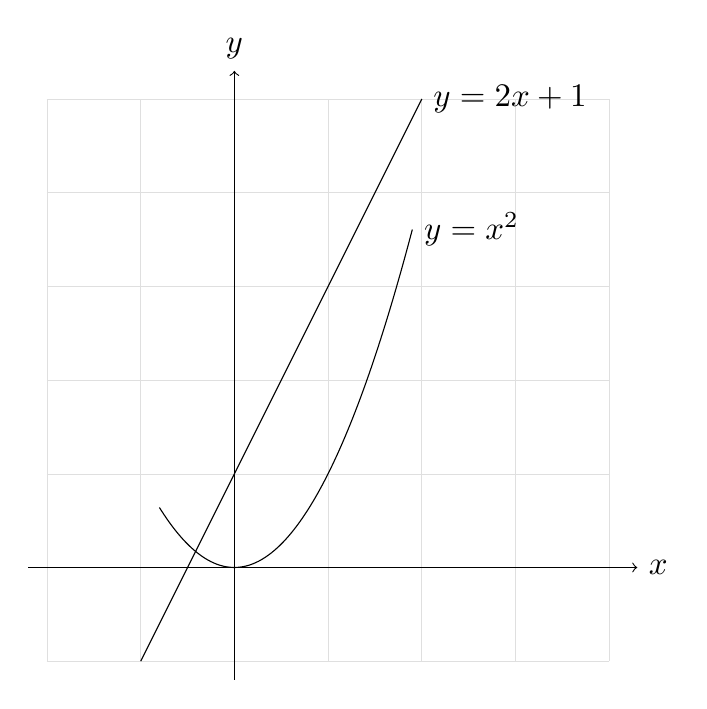
\begin{tikzpicture}[scale=1.19, transform shape]
    \draw[step=1, gray!25, very thin] (-2,-1) grid (4,5);
    \draw[->] (-2.2,0) -- (4.3,0) node[right] {$x$};
    \draw[->] (0,-1.2) -- (0,5.3) node[above] {$y$};
    \draw[domain=-0.8:1.9, smooth, samples=80] plot (\x,{\x*\x});
    \draw[domain=-1.0:2.0, smooth, samples=2] plot (\x,{2*\x+1});
    \node[right] at (1.9,3.61) {$y=x^2$};
    \node[right] at (2.0,5.0) {$y=2x+1$};
\end{tikzpicture}
